%-------------------------------------------------------------------------
\subsection{\upshape\textbf{Buckley-Leverett problem}}
\subsubsection*{\upshape\textbf{Theory}}
\hspace*{0.25cm}Buckley and Leverett [93] developed semi-analytical solution for
the displacement of two immiscible fluids in porous media.
Assuming constant fluid density (i.e. liquid flow), porosity, and
no source/sink terms the fluid mass balance equation can be
simplified.
\begin{equation}
n \frac{\partial S^\gamma }{\partial t} = - \nabla \cdot
\mathbf{q}^\gamma
\end{equation}
Buckley and Leverett derived the following expression
\begin{equation}
\frac{\partial S^l}{\partial f^l} = \frac{q_{tot}}{n} \frac{\Delta
t}{\Delta x}
\end{equation}
with the fractional flow function $f^\gamma = q^\gamma/q_{tot}$
\begin{equation}
f^1 = \left( 1 + \frac{\mu_1}{k_1} \frac{k_2}{\mu_2} \right)^{-1}
\end{equation}
1 and 2 are the fluid phase numbers. The position of the shock front separating the two fluid phases
can be calculated from the following expression.
\begin{equation}
\Delta x = - \frac{q_{tot}}{n} \frac{\partial f^l}{\partial S^l}
\end{equation}
\hspace*{0.25cm}Buckley and Leverett suggested that the capillary pressure is a
function of the saturation only. Note that the original
Buckley-Leverett considered the water and oil phase flow.
Moreover, they assumed that the condition that the derivative of
the capillary pressure with respect to the saturation is zero
$(dp_{cwo}/dp_{cwo}= 0)$ is a sufficient approximation that both
gradients of water and oil are equal each other.
\begin{equation}
\frac{\partial p_w }{\partial x} = \frac{\partial p_o}{\partial x}
+ \frac{\partial p_{cwo}}{\partial x} = \frac{\partial p_o
}{\partial x} + \frac{dp_{cwo}}{dS^w }\frac{\partial S^w}{\partial
x} = \frac{\partial p_o}{\partial x}
\end{equation}
\subsubsection*{\upshape\textbf{Problem definition}}
\hspace*{0.25cm} The Buckley Leverett problem is frequently used to test numerical models for the functional relation between relative permeability and saturation. In comparison to the analytical solution, the problem is simplified to describe one fluid displacing the other residing fluid in aquifers or reservoirs. In the derivation of the analytical solution, the effect caused by capillary forces between two fluids is not considered.

\hspace*{0.25cm} A non-wetting phase displaces a wetting phase from left to right. The initial total velocity of the two-phase system is $1.0 m/s$. The ratio of the dynamic viscosities is one, residual saturations are zero and the Brooks-Corey function ($\lambda = 2$) is used for the relative permeabilities. A space-time discretization of delta x = 0.025 m and delta $t = 0.005$. The total simulation time is $0.4 s$.
\subsubsection*{\upshape\textbf{PS-Global}}
\hspace*{0.25cm} Saturation equation, the mass conservation equation is converted to the volumetric one by dividing with fluids density.
\begin{align}
n\frac{{\partial S_{w}}}{{\partial t }} -
\nabla \cdot \left({\frac{{\mathbf k {k_{rel}}_w }}{{\mu_w }}\left( {\nabla p_w - \rho _w
\mathbf g} \right)} \right) = q_w
\label{eq:w_eqn}
\end{align}
\begin{align}
n\frac{{\partial S_{nw}}}{{\partial t }} -
\nabla \cdot \left({\frac{{\mathbf k {k_{rel}}_{nw} }}{{\mu_{nw} }}\left( {\nabla p_{nw} - \rho _{nw}\mathbf g} \right)} \right) = q_{nw}
\label{eq:nw_eqn}
\end{align}
A new BL result is obtained by GeoSys multiphase module that solves in a global-implicit scheme. As shown in the figure, the global-implicit scheme produces more accurate result compared to that obtained by the sequential-coupling scheme. The result has little oscillation and is closer to the analytical solution particularly in the location of the sharp front of the intruding fluid.


One thing important to note is that the global scheme is sensitive to matrix solvers. LIS solver (BiCG with Jacobi preconditioned) works on Windows. However, this iterative solver for this benchmark takes much more time than the PARDISO (a parallel direct solver) that works only on Unix with GeoSys.
\begin{figure}[!thb]
\begin{center}
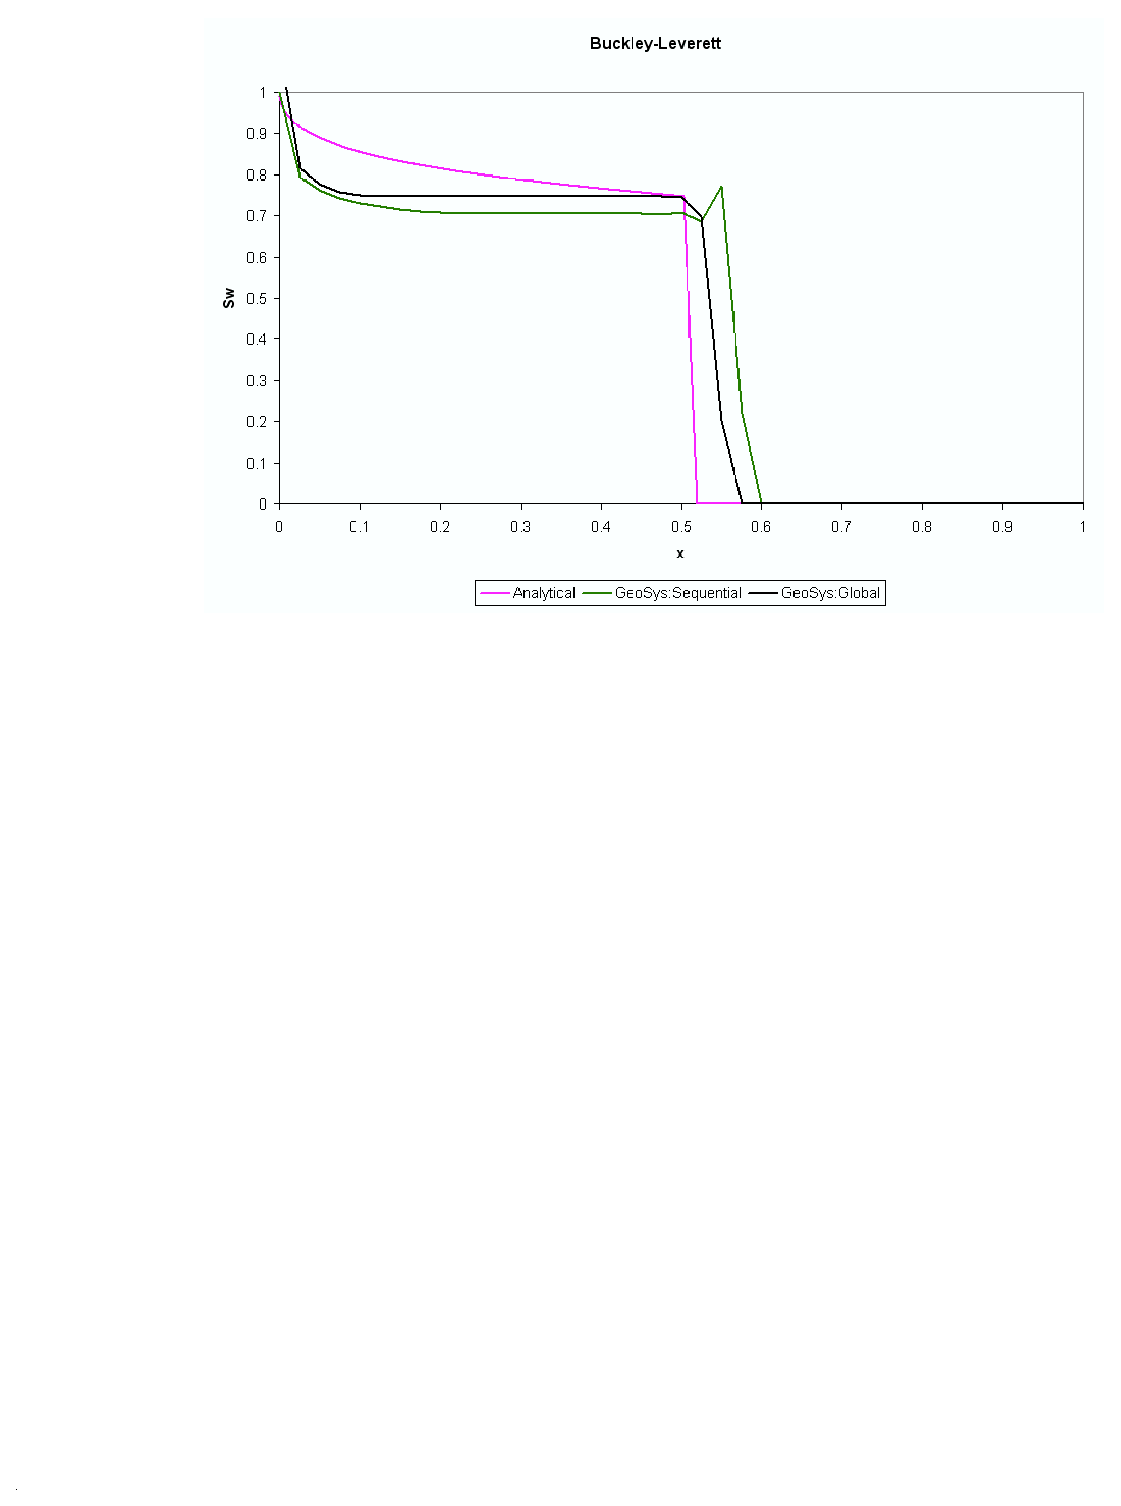
\includegraphics[scale=0.5]{HH/figures/PSGlobal.eps}
\end{center}
\vspace{-8.0cm}
\caption{}
\label{blg:comparison}
\end{figure}
\subsubsection*{\upshape\textbf{PS-Sequential}}
\hspace*{0.25cm}Adding (\ref{eq:w_eqn}) and (\ref{eq:nw_eqn}) with using the relation $S_{nw}+ S_w = 1$ and $p^{c}(S_w) = p_{nw} - p_w$, we get equation for wetting phase pressure, $p_{w}$ and non-wetting phase saturation, $S_{nw}$.
\begin{align}
 - n\frac{{\partial S_{nw}}}{{\partial t }} -
\nabla \cdot \left({\frac{{\mathbf k {k_{rel}}_w }}{{\mu_w }}\left( {\nabla p_w - \rho _w
\mathbf g} \right)} \right) = q_w
\label{eq:wfn_eqn}
\end{align}
\begin{align}
\nabla \cdot \left({\frac{{\mathbf k {k_{rel}}_w }}{{\mu_w }}\left( {\nabla p_w - \rho _w
\mathbf g} \right)} \right) +
\nabla \cdot \left({\frac{{\mathbf k {k_{rel}}_{nw} }}{{\mu_{nw} }}\left( {\nabla {p_w+p_c} - \rho _{nw}\mathbf g} \right)} \right) + \nonumber\\q_w + q_{nw} =0
\label{eq:nwfn_eqn}
\end{align}
In (\ref{eq:wfn_eqn}), non-wetting phase saturation, $S_{nw}$ can
be easily solved explicitly with the known pressure obtained from
(\ref{eq:nwfn_eqn}).

The analytical solution for the frontal location of the infiltrating fluid is derived and found there is the discrepancy with previous results (Helming and Huber $1998$, Figure $9$). In contrast to the previous results, the standard Galerkin-type method does tend to produce overestimated frontal infiltrating locations compared against the analytical solution. This can be explained by the diffusion term of the saturation originally omitted in the BL equation that makes purely advective transport. Handling this purely advective transport in general by the numerical models does introduces the numerical dispersion term naturally, and this added numerical dispersion can be interpreted by the saturation diffusion term.
\begin{figure}[!thb]
\begin{center}
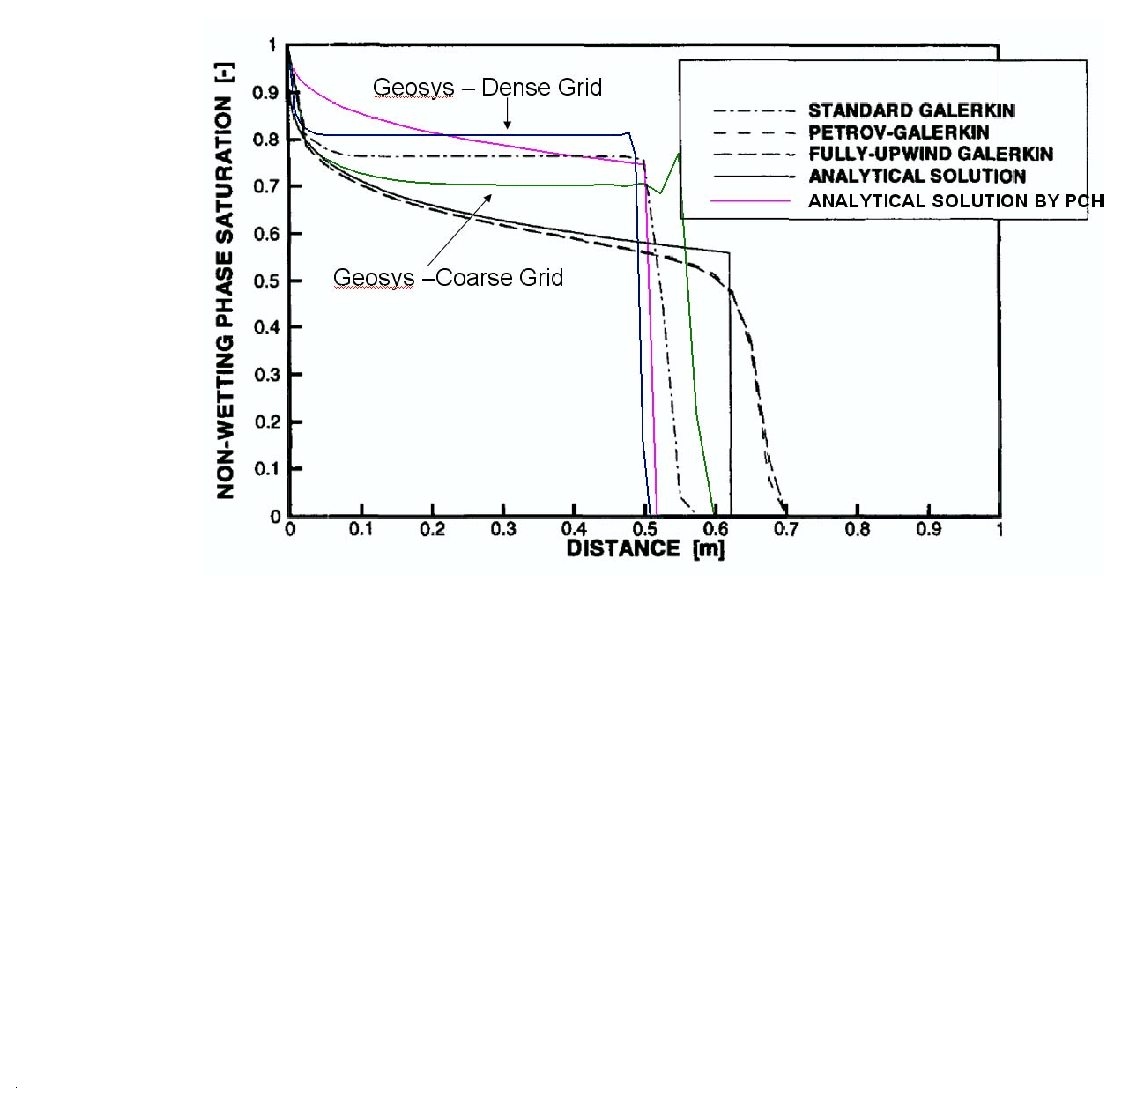
\includegraphics[scale=0.5]{HH/figures/PSSequential.eps}
\end{center}
\vspace{-5.0cm}
\caption{}
\label{bls:comparison}
\end{figure}
\subsubsection*{\upshape\textbf{Problem definition}}
\hspace*{0.25cm} Buckley and Leverett developed semi-analytical solution for the displacement of two immiscible fluid in porous media. Assume saturated $CO_2$ displacing $H_2O$ with constant fluid properties.
\subsubsection*{\upshape\textbf{Results}}
\hspace*{0.25cm} Here, we shown the saturation profile, $S_w$ in Fig. $18.1.7$ along $1~m$ column calculated with line element with space-time discretization of $\delta x = 0.025~m$ and $\delta t = 0.005~s$. The total simulation time is $0.4~s$; using the total-pressure-based pS-GLOBAL. Based on linear relation between saturation and relative permeability, saturation profile, $S_w$ is shown in Fig. $18.1.8$.\\\\
\begin{table}[!htb]
\begin{tabular}{lccr}
\hline\hline\noalign{\smallskip}
Property & Symbol & Value & Unit \\
\noalign{\smallskip}\hline\noalign{\smallskip}
Column length & $L$ & $m$ & $1.0$  \\
Porosity & $n$ & -- & $2.0\times10^{-1}$ \\
Permeability & $\kappa$ & $ m^2$ & $1.0\times 10^{-10}$ \\
Water dynamic viscosity &  $\mu_w$ & $Pa.s$ & $1.0\times10^{-3}$ \\
Gas dynamic viscosity & $\mu_{nw}$ & $Pa.s$ & $7.0343\times10^{-4}$ \\
Water density &  $\rho_w$ &$kg.m^{-3}$ & $1.0\times10^{3}$ \\
Gas density &  $\rho_{nw}$ & $kg.m^{-3}$ & $7.73\times10^{2}$ \\
Capillary pressure & $p^c(S)$ & $Pa$ & 0 \\
Relative permeability & $\kappa_{rel}(S)$ & -- & Brook-Corey functions \\
\noalign{\smallskip}\hline\hline
\end{tabular}
\caption{Material parameters for the BL problem.}
\end{table}
\begin{figure}[!thb]
\begin{center}
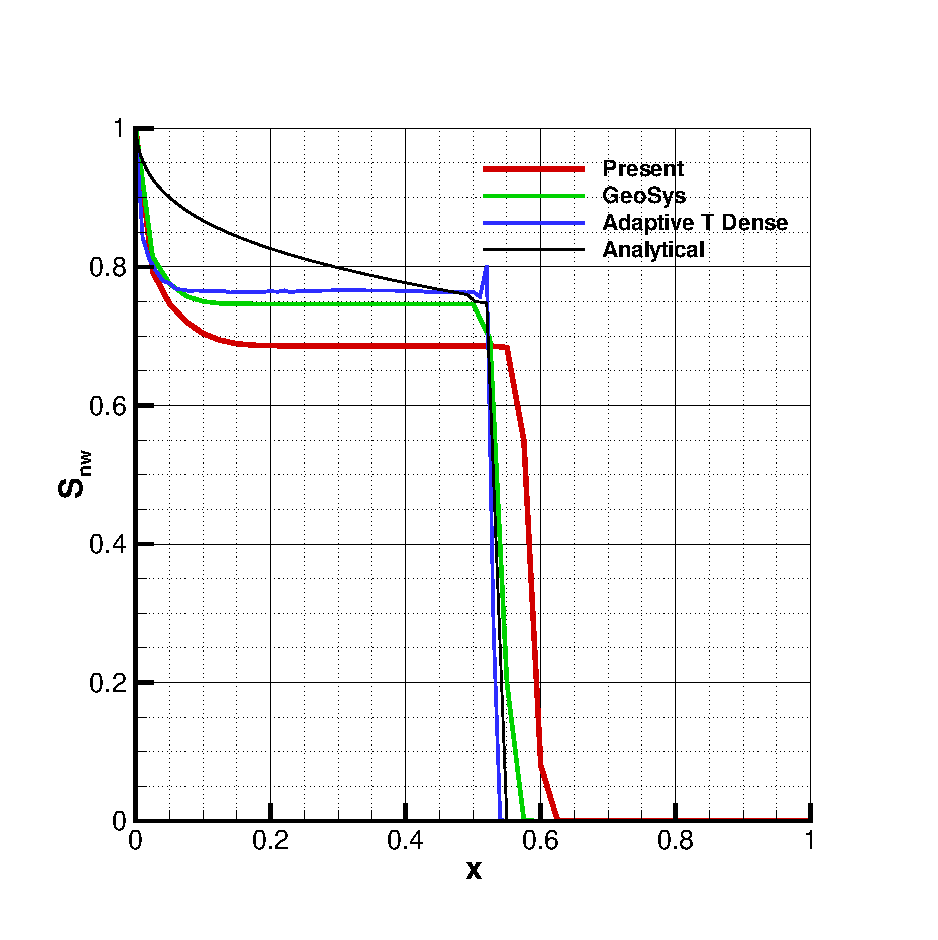
\includegraphics[scale=0.5]{HH/figures/BL-Sw.eps}
\end{center}
\caption{Saturation profile obtained with present analysis along with others.}
\label{bl:comparison}
\end{figure}
\begin{figure}[!thb]
\begin{center}
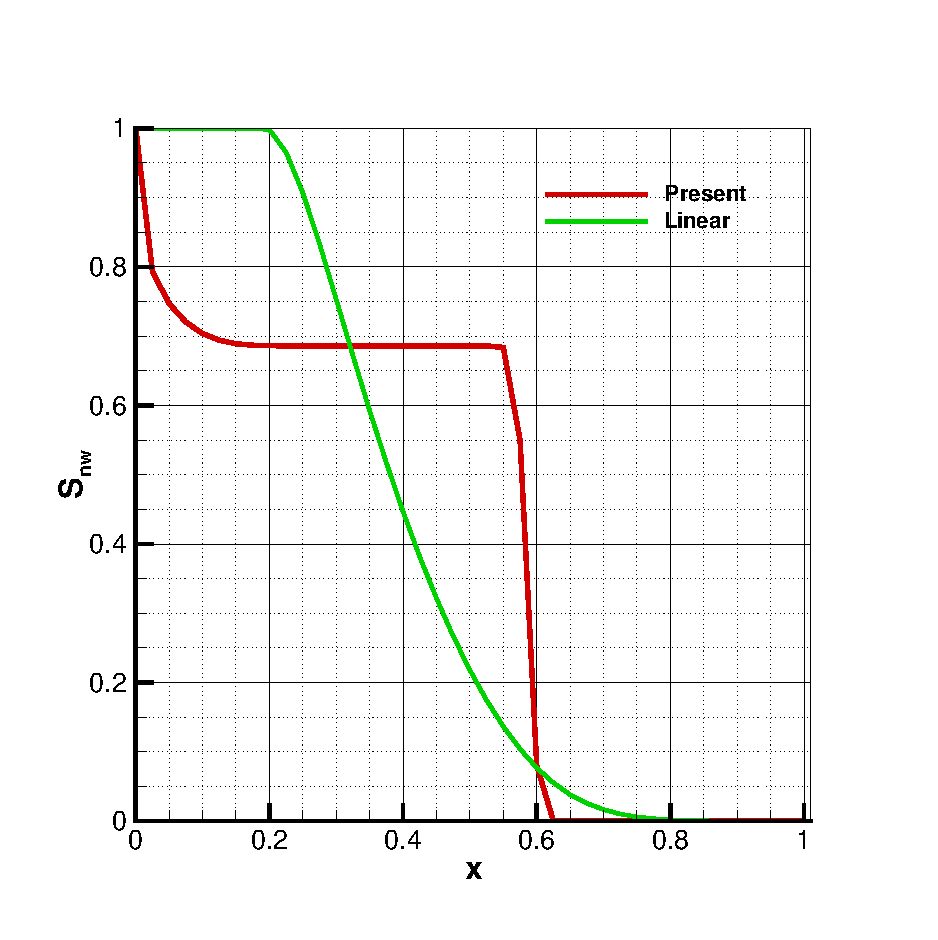
\includegraphics[scale=0.5]{HH/figures/BL-Sw-Linear.eps}
\end{center}
\caption{Saturation profile obtained with present analysis along with linear permeability and saturation relation.}
\label{bl:comparison}
\end{figure}
\clearpage
\subsubsection*{\upshape\textbf{Benchmark deposit}}
\begin{tabular}{|l|l|l|}
\hline
Benchmark & Problem type & Path in benchmark deposit \\
\hline
\emph{hm\_unsat}& HH & MULTIPHASE \\
\hline
\end{tabular}
\clearpage
